\section{Hasonló eszközök}

Egy hasonló rendszer már megvalósult \cite{similarSystem} ami egy Arduino\cite{ArduinoAtmega} 
mikroprocesszoron alapul. Ez egy egyszerűbb rendszer, ami csupán ellenállásokat használ az 
alkatrészek felismerésére és egy kijelzőt az adatok megjelenítésére. Ebből több fejlesztés is 
kialakult, több minden tesztelésére és nagyobb pontosság elérésére, miközben a rendszer 
egyszerűségét fenntartani. Ezek a rendszerek viszont nem használnak DAC-ot és ezért nem képesek 
karakterisztika diagramot készíteni. Ezen kívül nem csatlakoztatható egyszerűen számítógéphez, 
csupán újraprogramozás céljából, így minden esetben kell tartalmazzanak egy kijelzőt, ami 
növeli a költségeket. Az általános működésük hasonló, mint ebben a projektben, viszont itt 
precízen lehet változtatni a feszültséget, nem csak kapcsolni földre vagy tápfeszültségre.
Az bekötése hasonlóképpen történik: lásd \ref{fig:basicTesterConnection}

\begin{figure}[h]
    \centering
    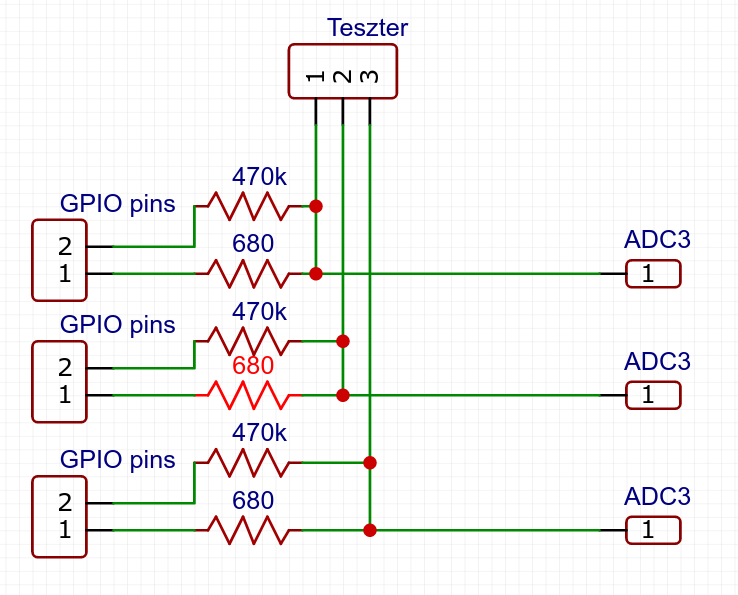
\includegraphics[scale=0.3]{figures/images/literature/OrgTesterConnection.png}
    \caption{Eredeti teszter bekötési rajza}
    \label{fig:basicTesterConnection}
\end{figure}

Mindegyik GPIO pin lehet csatolva földre, vagy tápfeszültségre, de le is lehet kapcsolva, így 
nem befolyásolja az áramkör működését. Az ADC pin meg lehet ADC üzemmódban, ilyenkor nem befolyásolja
az áramkört, viszont lehet földre, vagy tápfeszültségre is kapcsolni, ilyen esetben port ellenállás
nélkül csatolódik az áramkörre.

Viszont szintén hordozható egy 9V-os elem segítsségével és az eredmények megjelennek egy
kis LCD kijelzőn, ebből több féle verzió is létezik, van amely csak egy karakter kijelzőt
használ, van amelyik egy színes kép kirajzolására is alkalmas kijelzőt alkalmaz. 

A tesztelés néhány másodpercbe telik, nagy méretű kondenzátorok esetén telhet több időbe,
viszont ebben az esetben csak annyi idő, míg a legkissebb ellenálláson keresztül képes feltölteni
a kondenzátorot.


\section{Felhasznált technológiák}

A megvalósításhoz szükséges egy processzor, erre egy Raspberry pi pico \cite{RaspberryPico} 
mikrovezérlőt használtam. Erre a teljesítménye és alacsomy ára miatt került a választás.

%Ez egy olcső, miközben viszonylag nagy teljesítményű mikrovezérlő,
%2 hardwer szintű SPI \cite{SPIprotokol} csatornát és 3 darab 12 bites ADC-t tartalmaz.
%Erre a választás azért került, mivel még a terv kigondolása előtt már tulajdonomban volt. ,
%Hasonló mikrovezérlők vagy költségesebbek (pl. ESP32), vagy nagyon optimalizálni kellene a programot, 
%hogy ne lépje túl a hardver limitációjait (pl. Arduino).

A projekt tartalmaz egy ILI9341 \cite{ILI9341Datasheet} színes kijelzőt is, erre a nagy kijelző méret és 
nagy felbontás miatt esett a választás, hogy majd könnyedén látható legyen a mérés eredménye.

Ezen kívül használtam egy DAC8565 digital-alalóg átalakító, TS5A3357 analóg kapcsolót, és egy LP2950CZ-3.3
3.3V-os feszültség referenciát.

A rendszerher működéséhez szükséges egy 5V-os feszültség forrás, ez lehet egy általános USB
tápforrás, vagy lehetséges direkt 5V csatlakoztatása is. Az áramerősség alacsony, így nem közelíti
meg az 500mA-es áramerősség határt amit egy átlagos USB képes leadni. Külső akkumulátorról
is táplálható. Amennyiben egy számítógéphez, vagy egy olyan eszközhöz van csatolva ami képes 
a serial portot olvasni akkor a mérési eredményeket automatikusan elküldi azon keresztül a 
másik eszköz felé. 

A pontos részleteket az a következőkben lesznek leírva.

\section{A rendszer Blokk váza}
\begin{figure}[H]
    \centering
    \subfigure[A rendszer block váza]{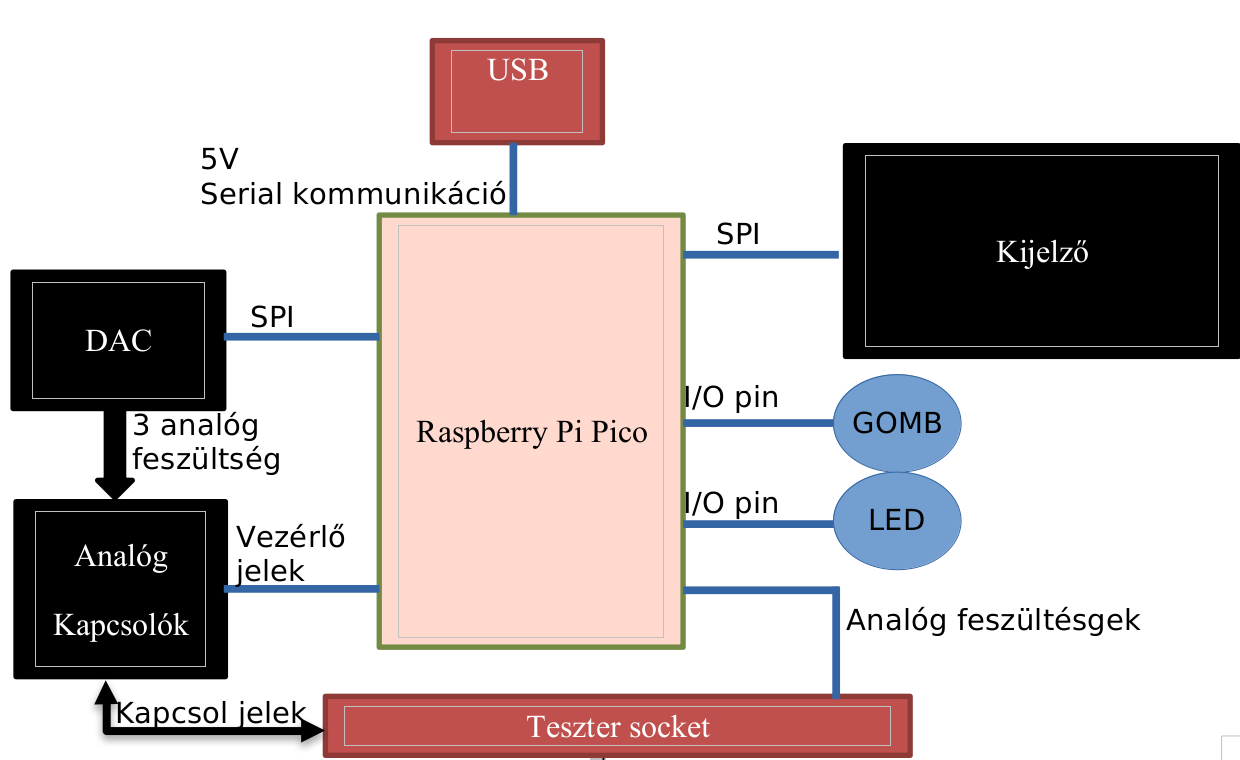
\includegraphics[scale=0.3]{figures/images/literature/blockDiagramm.png}}
    \caption{A rendszer block váza}
    \label{fig:blockDiagramm}
\end{figure}
